\subsection{Financial Markets}\label{subsec:assetprice}

% CDC: We can cite \cite{kuchler2021social} "social finance" survey and \cite{hirshleifer2020presidential} here.

% Quotes from \cite{kuchler2021social}:  Researchers have long understood that social interactions shape many aspects of economic activity. Yet, in most models of economics and finance, agents make financial decisions in a social vacuum in which prices are the only mechanism through which the actions of other agents affects beliefs and behaviors. This is likely to change substantially over the coming years. Indeed, the availability of new data has facilitated a recent surge of empirical research documenting large effects of so- cial interactions and processes on the economic and financial decisions of households and firms. Many of the documented effects are too large for theory to ignore, and early progress has been made in incorporating social interactions into equilibrium models of economic decision-making.

% Quotes from \cite{kuchler2021social}: First, social networks can serve as a source of actual or perceived information, and people might thus be influenced by their peers through a social learning channel, which can include the spread of both actual information as well as sentiments and beliefs (e.g., Bikhchandani, Hirshleifer & Welch 1992; Jackson 2010; Bailey et al. 2018a). The importance of social interactions in transmitting in- formation and beliefs in the household finance space is hardly surprising. Indeed, most people do not have much experience making important financial decisions such as buying a home, taking out a mortgage, or purchasing stocks. In addition, many possible sources of information, such as mortgage brokers and investment advisers, often have real or perceived conflicts of interest. As a result, it seems natural that individuals would turn to friends, colleagues, and family members— especially those with experiences relevant to the decision at hand—as trusted sources of advice.

% Quotes from \cite{hirshleifer2020presidential}: Social economics and finance recognizes that people observe each other and talk to each other, where talking includes written text and social media. A key but underexploited intellectual building block of social economics and finance is social transmission bias, the systematic directional modification of ideas or signals as they pass from person to person.

% Quotes frm \cite{hirshleifer2020presidential} Several authors propose that compartmental models from epidemiology can capture the spread of folk models and financial behavior. In such models, an infection with a financial belief, such as enthusiasm for a technical strategy or for Bitcoin, spreads through a population over time via random contacts. Some versions of compartmental models, such as the SIR Model, have an epidemic rise-and-fall time path. So the SIR Model has been applied to help explain trading and price bubbles.

% \begin{center}[Insert Figure \ref{fig:graph_investment}  here]\end{center}


\begin{figure}[!ht] \centering  % [h!]
  \caption{ ~Literature map of EE models of stock/housing market investment}
  \label{fig:graph_investment}
  \centerline{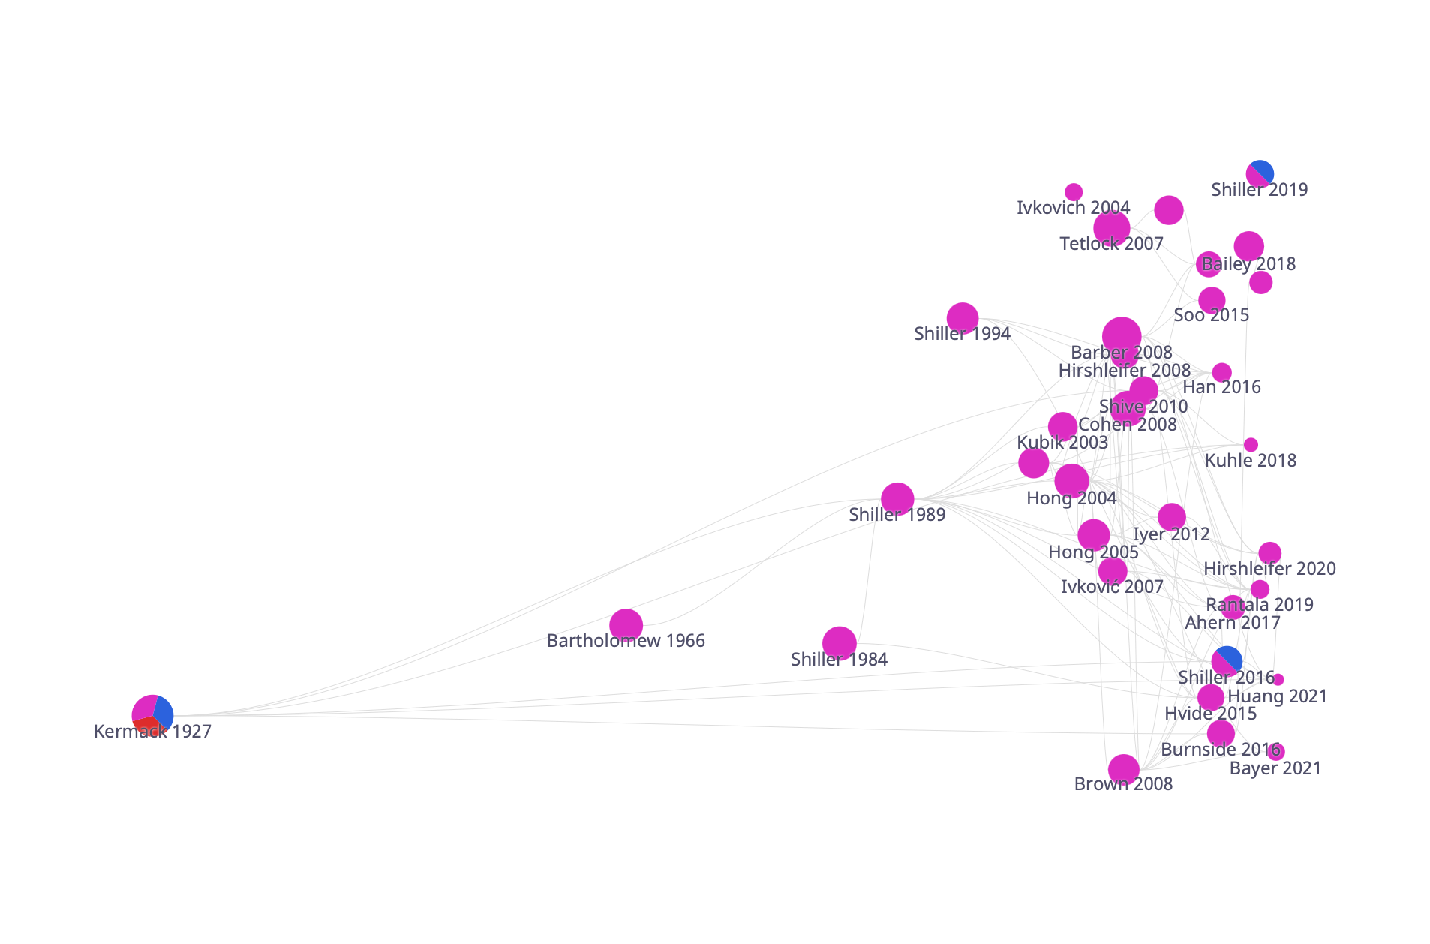
\includegraphics[width=0.9\textwidth]{./figures/graph_investment}}
  \begin{flushleft}
    {\footnotesize Note: This graph includes selected papers related to epidemiological models of expectations in asset markets, and studies of the role of news media in financial markets. See \href{https://app.litmaps.co/shared/E25276CA-8725-437B-8241-11961EFB3FB4}{here} for an interactive version.}
  \end{flushleft}
\end{figure}

Academic models of financial markets have traditionally assumed that investors choose stocks based on well-informed rational beliefs about future returns.  But popular treatments have emphasized social communication, and ideas with a distinctly epidemiological flavor, since the first published description of  the first publicly traded securities (\cite{vegaConfusion}'s discussion of the trading of shares of the East India company on the Amsterdam stock exchange).  \cite{mackay1850memoirs}'s vivid prose has made his (thoroughly epidemiological) descriptions of the Dutch Tulip mania and other financial episodes of ``The Madness of Crowds'' a classic of English literature.  This theme has continued to the present: Michael \cite{lewis2011big}'s bestselling book about the Great Financial Crisis goes so far as to suggest that one of the reasons a particular analyst was able to perceive the housing bubble early was his psychological indifference to other people's opinions.

The academic tide seems now to be turning toward an acknowledgment that there is some truth in the popular view. \cite{hirshleifer2020presidential}'s Presidential Address to the American Finance Association urged the profession take up the study of the social transmission of ideas as ``[a] key but underexploited intellectual building block of social economics and finance.''   Hirshleifer specifically points out the potential for epidemiological models to make sense of patterns that have been difficult to understand with traditional models.  \cite{kuchler2021social} propose `social finance' as the name for a field that would study such social interactions, and make a powerful case that new sources of data and new modeling techniques offer great promise.

These are by no means the first academic authors to propose a role for social transmission of financial ideas.  But, as we explained above, the proportion of efforts that could be described as constituting a full-fledged EE analysis, as opposed to piecemeal evidence or provocative theoretical exercises, is small. % (See Figure \ref{fig:graph_investment})

An early example of such a comprehensive approach is the paper by \cite{shiller1989survey} used above to delineate the elements of a standard epidemiological model.  \cite{shiller1989survey} constructed survey questions designed to understand the sources of information that motivated investors' initial interest in the stock that they had most recently purchased (which they designate as `randomly selected' -- \texttt{RAND}).  About a third indicated that their interest in that stock originated with ``a person who is not an investment professional.''  The authors identify another category of stocks owned by their survey respondents as ``rapidly rising'' and for those they find that roughly half of the initial interest in the stock originated with nonprofessionals.  Using a different methodology to designate `rapidly rising' -- `\texttt{RPI}' -- stocks for institutional investors, they find that 10 percent and 30 percent of their initial interest originated from `nonprofessionals.'

The survey-based estimates of their epidemiological model for both individual (`\texttt{IND}') and institutional (`\texttt{INS}') investors reveal considerable heterogeneity in infection rates both within and between the two groups. They also suggest that the infectiousness differs between a randomly selected stock \texttt{RAND} and a rapidly rising stock \texttt{RPI}. Interestingly, they find that the \texttt{RAND} category is more (interpersonally) ``infectious'' than the rapidly rising stock; they propose, plausibly, that public news sources will already have widely covered the rapidly rising stocks, so that interpersonal communications are unnecessary to bring attention to them.

Our Figure \ref{fig:sir_simulate} shows the compositional changes of investors under the paper's median estimates (of infection and removal rates) for individual and for institutional investors, and for randomly selected versus for rising stocks, respectively.\footnote{We convert all the continuous-time rates into discrete-time and from annual to weekly frequency. For instance, the recovery rate estimated from the decaying pattern of the time spent on studying a given stock for INSRPI is $g=1.39$ (a half-life of $ln(2)/g=0.50$ years). In discrete-time and at weekly frequency, this is equivalent to a probability of recovery $\gamma = 1-\exp^{-g/52} =0.02$. For the removal rate, under the assumption made by the paper that the fraction of susceptible is close to $1$ despite being time-varying, the estimated median removal rate of INSRPI is $b = 2.02$. It is converted to a weekly probability of $\beta = 1-\exp^{-b/52}=0.038$.}$^{,}$\footnote{We set the initial fraction of the infected to be $1$ percent.}

% \centerline{[Insert Figure \ref{fig:sir_simulate} here]}

\begin{verbatimwrite}{./Slides/FigureSIRSimulation}%%%Slides
  \begin{figure} \centering  % [h!]  [!ht]
    \caption{ ~Simulated dynamics from a SIR model of stock investors}
    \label{fig:sir_simulate}
    \centerline{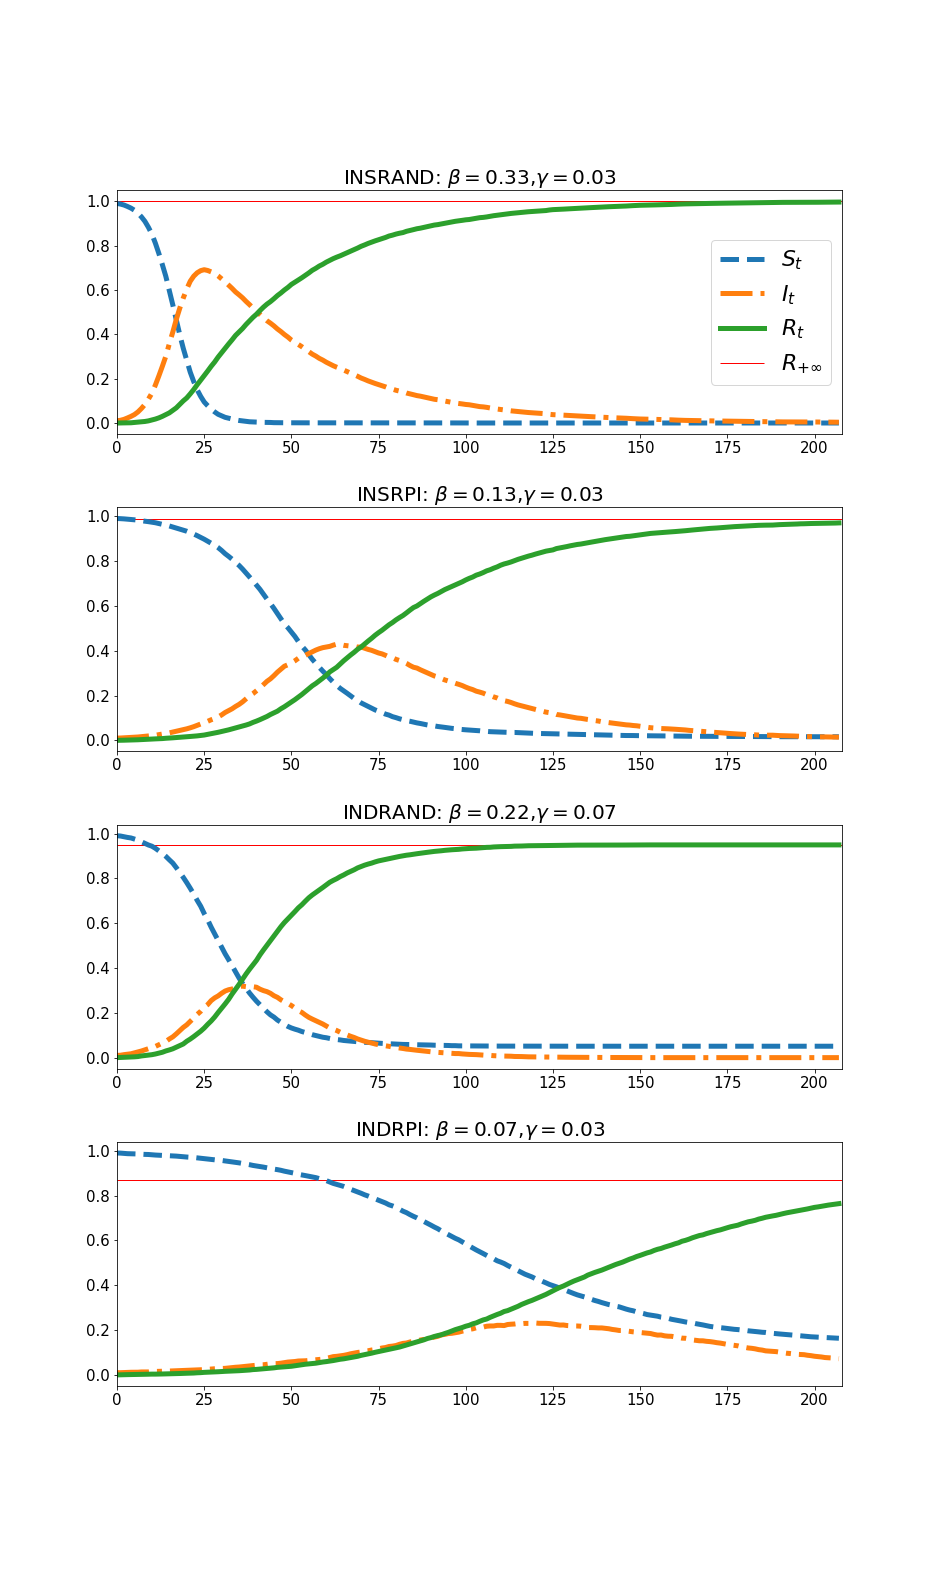
\includegraphics[width=0.85\textwidth,height=0.85\textheight]{./figures/sir_simulate}}
    \begin{flushleft}
      {\footnotesize Note: This graph plots the simulated paths of populations in different compartments in a SIR model of stock investors, as described in \cite{shiller1989survey}. We use the median estimates of the infection rate $\beta$ and recovery rate $\gamma$ for four samples: institutional investors for a randomly selected stock (INSRAND), institutional investors for a rapidly rising stock (INSRPI), individual investors for a random stock (INDRAND), and individual investors for a rapidly rising stock (INDRPI). The horizontal thin solid line corresponds to the limiting size of compartment of $R$ in the long run. The simulation is done with the Python library \href{https://ndlib.readthedocs.io/en/latest/}{``NDlib''}, for details, see the companion \href{https://github.com/llorracc/EpiExp/blob/master/SIR_Ndlib.ipynb}{Jupyter Notebook}. }
    \end{flushleft}
  \end{figure}
\end{verbatimwrite}%%%Slides
%%%Slides
  \begin{figure} \centering  % [h!]  [!ht]
    \caption{ ~Simulated dynamics from an SIR model of stock investors}
    \label{fig:sir_simulate}
    \centerline{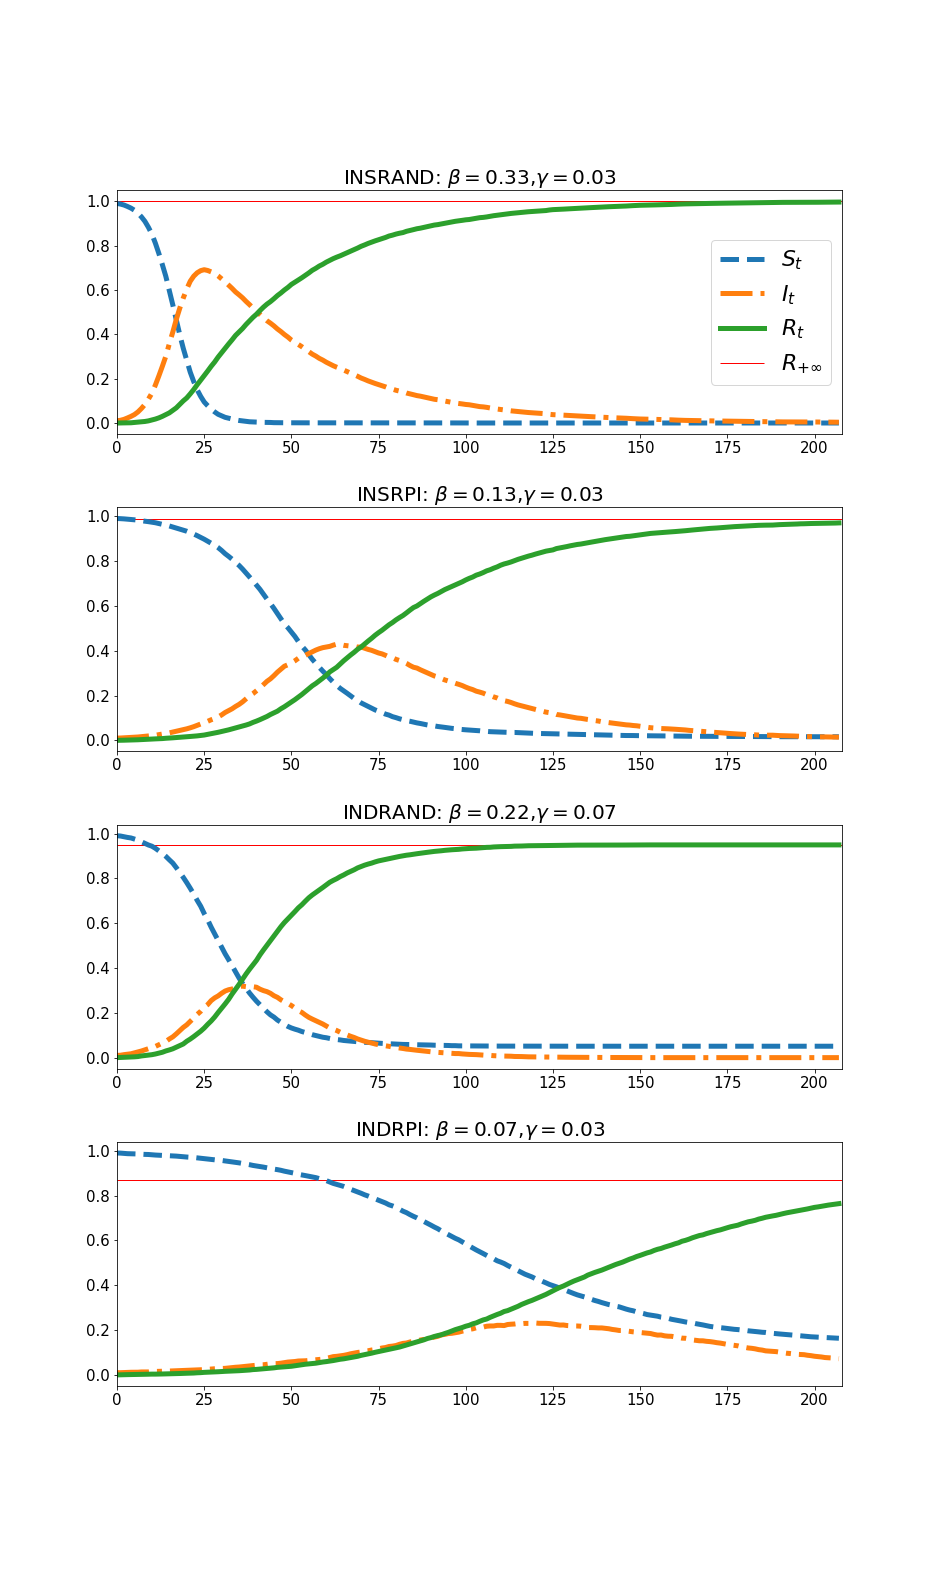
\includegraphics[width=0.85\textwidth,height=0.85\textheight]{./figures/sir_simulate}}
    \begin{flushleft}
      {\footnotesize Note: This graph plots the simulated paths of populations in different compartments in a SIR model of stock investors, as described in \cite{shiller1989survey}. We use the median estimates of the infection rate $\beta$ and recovery rate $\gamma$ for four samples: institutional investors for a randomly selected stock (INSRAND), institutional investors for a rapidly rising stock (INSRPI), individual investors for a random stock (INDRAND), and individual investors for a rapidly rising stock (INDRPI). The horizontal thin solid line corresponds to the limiting size of compartment of $R$ in the long run. The simulation is done with the Python library \href{https://ndlib.readthedocs.io/en/latest/}{``NDlib''}, for details, see the companion \href{https://github.com/llorracc/EpiExp/blob/master/SIR_Ndlib.ipynb}{Jupyter Notebook}. }
    \end{flushleft}
  \end{figure}
%%%Slides

The epidemiological analysis above is for parameters that characterize a sample of highly interested and motivated investors.  There is no sense in which these parameters can be thought of as characterizing the whole population -- which is why it is not as surprising or implausible as it might seem that all the parameterizations of the models were ones in which $\Recovered$ (the proportion of investors who would eventually become interested in a stock) was high.

The economic analysis can now also be interpreted in temporal terms.  The authors point out that a fully rational model with no private information would imply that trading volume should be heavily concentrated around identifiable dates of news events, but the epidemiological model is consistent with long and variable lags.  It takes around half a year for the interest of institutional investors in the randomly selected stocks to reach its peak and a little more than a year for a rapidly rising stock. As for individual investors, the population interested in \texttt{RAND} reaches its peak after 40 weeks, while interest in \texttt{RPI} takes 2.5 years to peak.


% sAlthough such paths correspond to a particular set of configurations, they presumably shed light on the general evolution patterns of stock investors' interests.  For instance, so long as the infection rate is higher than the removal rate, the fraction of infected investors will follow a hump shape  -- because the number of susceptible persons is declining.

The paper also argues that in a special case where the infection rate is close to the removal rate, and the size of the pool of interested investors is driven by serially uncorrelated shocks, stock prices could follow a random walk, because under those assumptions the change in the level of `interest' is nearly unforecastable.\footnote{\cite{shiller1984stock} presents an  elaboration on this logic by allowing the presence of both rational investors (``smart money'') and social-dynamics driven investors. The presence of unforecastable social dynamics weakens the statistical power of the random-walk test of rationality of stock market.} This is another example of an economic consequence flowing from the pattern of spread of an infection.  Furthermore, the pool of investors is potentially measurable, so it is an implication that can be tested.

Remarkably little of the extensive literature citing \cite{shiller1989survey} has involved meaningful epidemiological modeling; almost all of it has either been empirical, or has used a modeling framework that cannot be characterized as `epidemiological' as we are interpreting the term. %in Section \ref{subsec:epi_framework}.

A potential reason for this lack of followup is the nonexistence, until quite recently, of much direct data on either of the two key components of the model: beliefs (about, say, stock prices), or social connections -- and no data at all about the \textit{changes} of beliefs as a function of the structure of a measured social network.  \cite{shiller1989survey} had to make heroic assumptions in order to quantify their model.  Few subsequent scholars seem to have been willing to go so far in employing what might today be termed an `indirect inference' approach: ``Assuming the epidemiological model is right, let's calibrate it using its downstream implications for things we can observe.''

However, we have found two good exceptions, both of which estimate parameters of structural epidemiological model of stock investors using microdata.

The first is  \href{https://github.com/iworld1991/EpiExp/blob/master/Literature/shive2010epidemic.pdf}{\cite{shive2010epidemic}}, which uses an SI (`susceptible-infected') model to inform the structure of a reduced-form regressor that aims to capture social influences among investors.  Using nearly the universe of ownership data for Finnish stocks between 1994 and 2004, the author assumes that the key social infection channels are at the municipal level, and estimates the time-series dynamics of ownership within municipalities.

Specifically, controlling for all of the variables (demographic variables, news sources, price dynamics, and others) that standard models might suggest could affect ownership patterns, the author estimates an equation that can be interpreted as measuring the $\beta$ coefficient in Equation~\eqref{eq:sirdyn}.  The estimated $\beta$ coefficient is highly statistically significant, indicating at a minimum that there is some local dynamic pattern to stock purchases not captured by the usual finance and economic models, but which is captured by `proportion locally infected last period' (corresponding to $S_t/N$ in Equation~\eqref{eq:sirdyn}).  % An epidemiological interpretation of this fact seems quite natural.

The second example is \href{https://github.com/iworld1991/EpiExp/blob/master/Literature/huang2021rate.pdf}{ \cite{huang2021rate}}, which estimates an epidemiological model of diffusion of financial news among geographical neighbors. The paper reports a time-average estimate of the reproduction ratio $\mathcal{R}$ between $0.3$ to $0.4$ (equivalent to $\frac{\beta S_t/N}{\gamma}$ in an SIR model); that is, each stock trade that the authors identify as exogenous (see the paper for the mechanism) resulted in a total of $0.3{\sim}0.4$ trades among that person's neighbors, aggregated over all neighbors and all time.

The authors also find stronger transmission between investors of the same characteristics (age, income category, and gender), confirming the usual presumption of homophily (people tend to trust others with similar backgrounds). The paper found stronger transmission between senders and receivers with high past performance, suggesting that conversations between neighbors were more likely when past performance has been high.  The natural interpretation -- consistent with common findings in behavioral finance -- is that you are more likely to boast about your investment in a winner than admit to having invested in a loser.

Their estimate that $\mathcal{R}$ is positive and highly statistically significant is consistent with the presence of neighborly social influence, and they work hard to rule out plausible alternatives. But since the estimated reproduction ratio is below  1, their results imply that news of this kind does not lead to an epidemic of stock trading.  This is in contrast with \cite{shiller1989survey}, whose corresponding reproduction ratios far exceeded one.  This difference highlights the extent to which epidemiological models must be interpreted with care; even if similar phenomena (stock trading) are being studied, and even if there is evidence of social communication, the estimated nature and size of the epidemiological consequences can vary greatly depending on the exact experiment.

A final, and very impressive, contribution that satisfies all our criteria is a model of housing market fluctuations by \href{https://www.journals.uchicago.edu/doi/abs/10.1086/686732}{\cite{burnside_understanding_2016}}, which shows how incorporating social interactions can generate booms and busts. In the model, agents differ in their beliefs (optimistic or skeptical) about the fundamental value of housing.  Although it is a random-mixing model, paper has a mechanism similar in its implications to the simplest epidemiological model of `super-spreaders' which occurs when some agents have many more social connections than others:  The agents in this model differ in the degree of confidence they have in their opinions (whether optimistic or pessimistic) and those with greater confidence are more likely to convert those who have less confidence.  Defining a `boom' as a period in which house prices rise rapidly as the result of a spread in optimism, and a `bust' as a rapid decline in prices caused by rising proportion of skepticism, their most interesting result is that whether a boom is followed by a bust can depend on whose opinion (optimists or skeptics) turns out to be closer to the true fundamental value.  Specifically, busts happen when the skeptics turn out to be right about the fundamentals, while booms caused by optimists who happen to be right are not followed by busts.

One further literature that deserves a brief mention is the work on ``Agent Based Computational Finance'' (see the survey of that title by~\cite{lebaronAgentCompFinance}).  It would be straightforward to reinterpret much of the work in that literature as exploring epidemiological models of expectations of asset prices and financial market outcomes, and epidemiological terminology is sometimes explicitly invoked in the literature.  Economists interested in constructing formal EE models would do well to delve into that literature for ideas that could be reinterpreted (or relabeled) to purpose.  We have chosen not to survey that literature here partly because there are a number of excellent surveys already available, and in part because that literature has not mainly interpreted itself as modeling the dynamics of expectations.